% --------------------------------------------------------------
% This is all preamble stuff that you don't have to worry about.
% Head down to where it says "Start here"
% --------------------------------------------------------------

\documentclass[10pt]{article}


\usepackage{graphicx,url}
\usepackage{proof}
\usepackage{framed}
\usepackage{etaremune}

\usepackage[margin=1in]{geometry}
\usepackage{amsmath,amsthm,amssymb,amsfonts}
\usepackage{paralist}

\usepackage[most]{tcolorbox}

\definecolor{bg}{rgb}{0.9,0.9,0.9}%-- try others later
\definecolor{lightgray}{rgb}{0.95,0.95,0.95}%-- try others later
\definecolor{block-gray}{gray}{0.9}%-- try others later
\definecolor{dark-gray}{gray}{0.86} %-- try others later
\definecolor{light-gray}{gray}{0.96} %-- try others later
\newtcolorbox{myquote}{colback=block-gray,breakable,boxrule=0pt}
\newtcolorbox{mydarkquote}{colback=dark-gray,breakable,boxrule=0pt}
\newtcolorbox{mylightquote}{colback=light-gray,breakable,boxrule=0pt}


% 1. To get version suitable for students to populate,
%    remove the contents of the \ignoreSoln{..body..}
%
% 2. To get a version suitable for generating PDF 
%    without solutions, remove the #1 below
%
% 3. To generate solutions, keep the #1 below
%
% 4. Assigned grader fills \ignoreSoln{..body..}
%    and also provides his/her feedback to student
%    and policy followed for point deduction
%    So design policy before grading begins.

\newcommand{\ignoreSoln}[1]{#1}   
%\newcommand{\ignoreModel}[1]{#1} 


\newcommand{\bigset}[2]{\big\{\;#1\;:\;#2\;\big\}}
\newcommand{\N}{\mathbb{N}}
\newcommand{\Z}{\mathbb{Z}}
\newcommand{\R}{\mathbb{R}}
\newcommand{\Np}{\mathbb{N^{+}}}

\newenvironment{theorem}[2][Theorem]{\begin{trivlist}
\item[\hskip \labelsep {\bfseries #1}\hskip \labelsep {\bfseries #2.}]}{\end{trivlist}}
\newenvironment{lemma}[2][Lemma]{\begin{trivlist}
\item[\hskip \labelsep {\bfseries #1}\hskip \labelsep {\bfseries #2.}]}{\end{trivlist}}
\newenvironment{exercise}[2][Exercise]{\begin{trivlist}
\item[\hskip \labelsep {\bfseries #1}\hskip \labelsep {\bfseries #2.}]}{\end{trivlist}}
\newenvironment{reflection}[2][Reflection]{\begin{trivlist}
\item[\hskip \labelsep {\bfseries #1}\hskip \labelsep {\bfseries #2.}]}{\end{trivlist}}
\newenvironment{proposition}[2][Proposition]{\begin{trivlist}
\item[\hskip \labelsep {\bfseries #1}\hskip \labelsep {\bfseries #2.}]}{\end{trivlist}}
\newenvironment{corollary}[2][Corollary]{\begin{trivlist}
\item[\hskip \labelsep {\bfseries #1}\hskip \labelsep {\bfseries #2.}]}{\end{trivlist}}

\DeclareMathSizes{14}{14}{14}{14}

\begin{document}

% --------------------------------------------------------------
%                         Start here
% --------------------------------------------------------------

%\renewcommand{\qedsymbol}{\filledbox}


\begin{center}
\begin{large}
  CS 3100, Spring 2020, \\
  Final Battery of Problems (solutions, if present, in {\sf sf font}) \\
  (These will be adapted for Canvas)
\end{large}
\end{center}

\date{}


\vspace{1ex}

\section{WHAT IS ON Midterm-3?}

\noindent    Midterm-3 will consist of

\begin{itemize}
\item The basics of TMs from Chapter 13, asked as multiple-choice questions.
  \begin{itemize}
  \item Simple properties of TMs such as its input and tape alphabet
  \item Language of a TM
  \end{itemize}

\item The design of a simple TM (much simpler than what was asked in Asg-6)

\item Asg-6 (whose solutions will be posted online)
  
\end{itemize}

\vspace{1ex}

\section{WHAT IS ON THE FINALS?}

\noindent Asg-7 and simple questions covering the whole course.

\begin{itemize}
\item The basics of TMs from Chapter 13, asked as multiple-choice questions.
  \begin{itemize}
  \item Simple properties of TMs such as its input and tape alphabet
  \end{itemize}
\end{itemize}


\section{PROBLEMS}

\noindent Questions below give you practice pertaining to Asg-6 and Asg-7.

\begin{enumerate}
\item Is $\emptyset$ recursive?
\item[] {\sf Answer yes. There is an algorithmic membership test. Algorithm: always return false.}
\item[]
  
\item Is $\{1,2,3\}$ recursive?
\item[] {\sf Answer yes. Implement a C function (or TM) that given 1 or 2 or 3 returns True else False.}

\item Is $LanguageOf(0*1*)$ recursive?
\item[] {\sf Answer yes. Implement a pattern matcher that matches for that regexp.}
\item[]

\item Is $LanguageOf(CFG\; G)$ recursive?
\item[] {\sf Answer yes. Implement a parser for $G$.}
\item[]

\item Is $LanguageOf(PDA\; P)$ recursive?
\item[] {\sf Answer yes. Run the pda on the given membership test string.}
\item[]  

\item Is $LanguageOf(TM\; M)$ recursive?
\item[] {\sf Answer no.} The proof that $A_{TM}$ being not recursive, from first principles. (We build the $D$ machine
   and ask what happens to $D(D)$.)
\item[]  

\item Is $LanguageOf(TM\; M)$ RE?
\item[] {\sf Answer yes.} Dovetail list strings from
  $\Sigma^*$ and run $M$ in tiny increments of fuel (ever-increasing) on those strings. Whenever
  $M$ accepts a string, list that string. That enumerates the language of $M$.
\item[]

\item Is the language called $A_{TM}$ RE?
\item[] {\sf Answer yes.} Dovetail list pairs of strings from $\Sigma^*$
  such that the first pair is a Turing machine (or C program) $M$ and the second is $w$.
  $M$ in tiny increments of fuel (ever-increasing) on $w$. Keep doing this for various $M$ and $w$.
  Whenever
  $M$ accepts some string $w$, list that pair That enumerates the language of $A_{TM}$.
\item[]    
\end{enumerate}

\subsection{The language hierarchy}



\begin{center}
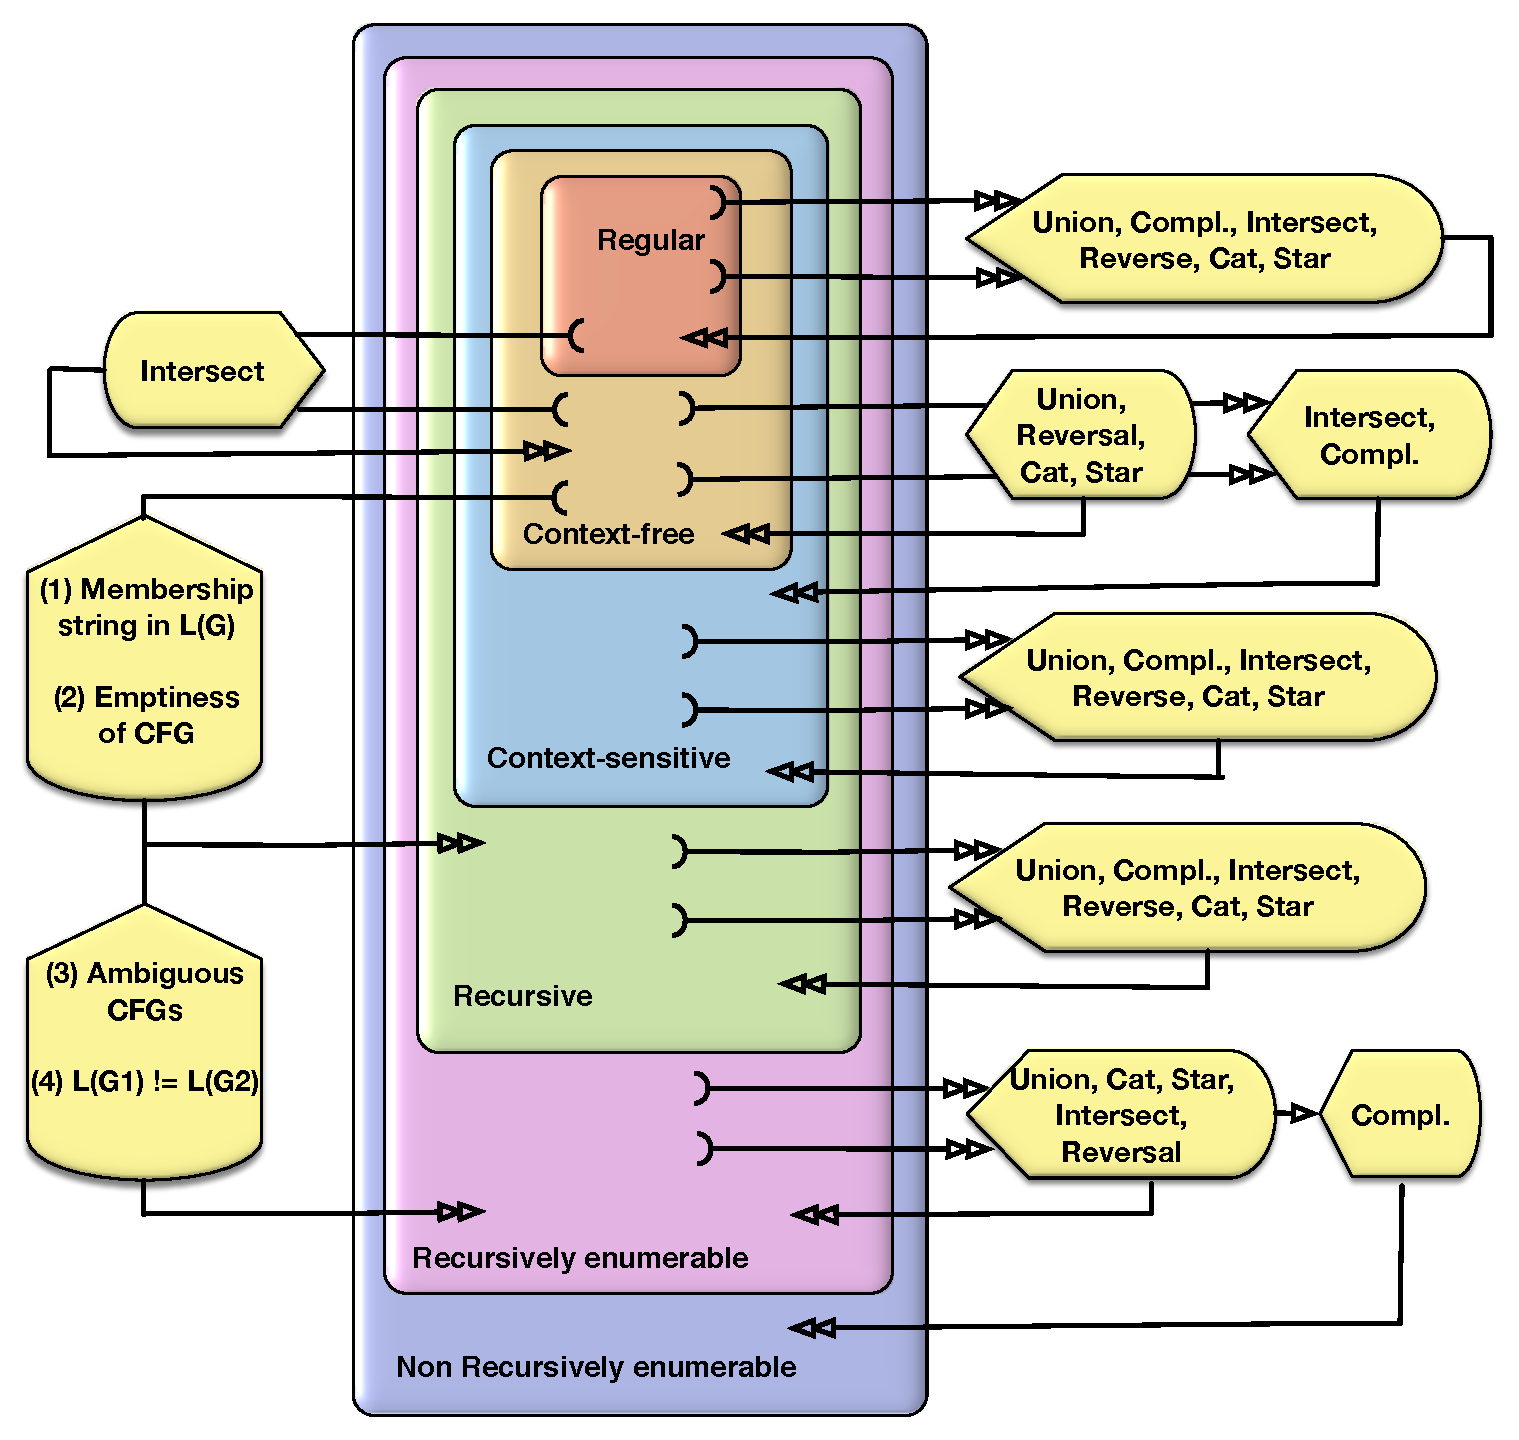
\includegraphics[angle=0,width=.5\linewidth]{DecidabilityDiagram.pdf}
\end{center}


\begin{enumerate}
\item Given the language hierarchy (Figure 14.2, Section 14.4,
  reproduced on this page),
  answer the following:
  \begin{enumerate}
  \item Is \( L_{emptycfg} =
    \{ \langle G\rangle \;:\; L(G)=\emptyset \}\) recursive? Here,
    $G$ is a CFG.

    \begin{enumerate}
    \item[] {\sf Answer: Yes. Keep sweeping from the start symbol of $G$
      to see if $G$ gets caught up in infinite recursion. Actually sweep
      from the terminals back to the $S$ (start) symbol of $G$. Somehow
      if $G$ manages to produce any string $s$ at all, then $L(G)\neq\emptyset$.
      Else it is equal to $\emptyset$.
      }
    \end{enumerate}

  \item Is \( L_{G1eqG2} =
    \{ \langle G_1,G_2\rangle \;:\; L(G_1)= L(G_2) \}\) RE, where
    $G_1$ and $G_2$
    are CFGs?

    \begin{enumerate}
    \item[] {\sf Answer: No.
      If you find a string $w$ accepted by one grammar but not the other, then
      the grammars are not language-equivalent.
      But if you keep finding all $w$ within the language of both grammars, you can't stop.
      Intuitively, grammar equality is not established with one string accepted by both.
      One has to ``exhaust'' all strings.
      The formal proof was discussed as a canvas response but not needed.
      }
    \end{enumerate}    
    
  \end{enumerate}
  
\item From the language hierarchy,
  we notice that  regular languages are contained
  in the family of context-free languages,
  but not vice-versa. On the other hand,
    the set $\Sigma^*$ is
    regular,
    and every CFL is a subset of this regular language.
    Explain!
    \begin{enumerate}
    \item[] {\sf Answer: One talks about language inclusion, the other
      talks about string inclusion.}
    \end{enumerate}
    
  \item Prove that there exist non-RE languages.
    \begin{sf}
      Argue how each RE language can be represented by a bit-vector, calling
      the bits

      \begin{footnotesize}
\begin{verbatim}
L0  b00 b01 b01 ...
L1  b10 b11 b12 ...
L2  b21 b22 ...
L3 ...
\end{verbatim}
      \end{footnotesize}
      Now consider the complemented diagonal. Write it out. Argue
      how it compares with each of the languages L0, L1, ...
    \end{sf}
    \begin{enumerate}
    \item[] {\sf Detailed Answer: Attempt to show that all TMs can be
      ``numbered'' (listed out). Thus, all the RE languages can be numbered.
      That is what I mean by L0, L1, L2, ... above.
      But now, one can find ONE language not in ANY of these languages.
      This is discussed in Appendix-C of the book (last ``chapter'').}
    \end{enumerate}


  \item How to write a proof for a language $L$ being RE.
    
  \item[] {\sf Answer: In general, state an approach to list $L$ via
    an enumerator Turing machine $M$.}
    %
  Assume that the notion of ``dovetail order''
  is well defined. Then, here is the pseudo-code for
  listing the language of TM M, which is the TM whose language L is:

\begin{verbatim}
For TM M whose language is an RE set, here is how we enumerate its language:

// Enumerate the language of a TM called M
//
TM_enumerator(M) {
<fuel,enumLen> = <0,0>;
//we advance in dovetail order i.e. 00,01,10,02,11,20,...
// i.e. all pairs that add up to N, then pairs that add up to N+1..
 forever do {
  generate next <fuel,enumLen> in dovetail order;
  for each x in Sigma* upto enumLen in numeric order
    { run M(x) with fuel;
      if M accepts x, print x;
    }
 }
}
// We would run M on every x in Sigma* for every amount of fuel
// If at all x in the language of M, we will discover it via this enumeration
\end{verbatim}


  
%  \begin{enumerate}
%  \item Prove that the set
%    %    $\langle \rangle$
%    $\langle Y\rangle$ of $Y$ combinators in
%    Lambda calculus is RE.
%
%  \item[] Solution: 
%    \begin{enumerate}
%    \item Enumerate all possible Lambda expressions $X$ that are
%      functions (lambda abstractions).
%
%    \item Apply $X$ to a function symbol $f$.
%
%    \item See if we can reduce $(X\; f)$ and
%      $f(X\; f)$ to a common normal form.
%
%    \item Whenever this happens, $X$ is a ``$Y$ combinator''
%      (fixpoint finder).
%    \end{enumerate}
%  
%  \end{enumerate}
  
\item How to write a proof for a language $L$ being recursive.
\item[] {\sf Answer: In general, state the algorithm, or state how one can
  enumerate $L$ and its complement.}

\item  
  \begin{enumerate}
  \item Prove that the set of Turing  machines $T$ that halt when
    started with input string $w$, and
    that do not write outside of positions $p_1$
    and $p_2$ on the tape ($p_1\leq p_2$) is recursive.
  \item[]
    \begin{sf}
      Answer:
    \begin{enumerate}
    \item Notice that the TM is not allowed to write more than
      a finite number of cells.
    \item Keep simulating this TM, observing the IDs attained
      by the TM.
    \item The number of IDs is finite. So when the IDs begin repeating
      and the TM has not yet halted, we can conclude that the
      TM will never halt.
    \item Following the aforesaid algorithm, we can conclude
      that this set of $\langle T,w,p_1,p_2\rangle$ is recursive.
    \end{enumerate}
    \end{sf}
    
  \item Prove that given an initial chessboard (pieces placed
    as usual) and a final checkmate position $P$, the moves
    (a string $m$)
    necessary to attain such a checkmate are decidable.
    That is, this language is recursive:
    \[ \{ \langle P,m\rangle \;:\; P\; {\rm }
    \; {\rm is}
    \; {\rm a}
    \; {\rm checkmate}
    \; {\rm achieved}
    \; {\rm via}
    \; m
    \}
    \]
  \end{enumerate}
    \begin{sf}
      Answer: Chess moves can be algorithmically checked.
    \end{sf}
    
    
\item \label{qn:intersect}
  Are RE sets closed under complementation?
  \begin{sf}
    Answer:
    
    If an arbitrary set (or language) $S$
  is RE and also $\overline{S}$ is RE (assuming closure under
  complementation), then we can enumerate $S$
  and $\overline{S}$ and decide membership of any given string in
  $S$  or $\overline{S}$. This makes $S$ recursive.
  
  Now answer this question. $S$ is an arbitrary set. Is any
  arbitrary set recursive? {\sf Answer: No! $A_{M}$ is not.}

  RE sets are closed under union, concatenation, intersection, reversal.
  Here is a taste for one proof (closure under intersection); write the others:

  \begin{sf}
    Answer:
  \begin{itemize}
  \item Define the following TM that takes $M_1$ and $M_2$:
      \begin{itemize}
  \item intersectM1M2($M_1$,$M_2$):
  \item run $M_1$ and $M_2$ in dovetail order on inputs, also
    generated by the dovetail enumeration procedure
  \item When this simulation notices $M_1$ and $M_2$ accepting
    some string, it emits that string
  \item This procedure now lists all strings in $M_1$ and $M_2$.
      \end{itemize}
  \end{itemize}
  \end{sf}
  \end{sf}

\item[] To recap, if a set $S$ and its complement $\overline{S}$
  are RE, then both $S$ and $\overline{S}$ are also recursive.
  Also, every
  recursive set is RE.


\item Show that the
  acceptance problem is undecidable (not recursive), but the language
    $A_{TM}$ is RE.
  Also, the
  Halting problem is undecidable, but the language
  $Halt_{TM}$ is RE.
  \begin{sf}
    Answer:
    The RE part is shown by defining an enumeration
    as in Question~\ref{qn:intersect}.
    The undecidable part is by the diagonal machine ``D'' or the
    corresponding diagonal machine ``E'' defined
    during Lecture 26 on Tuesday, Nov 27th.
  \end{sf}

\item Direct proof by contradiction of $A_{TM}$ being undecidable, using
  $Halt_{TM}$ being undecidable as the ``old existing undecidable problem.''
  \begin{sf}
    Answer:
    Review the ``boxes within boxes'' construction that involved
    the two boxes for $A_{TM}$ and the ``edit'' feature.
  \end{sf}

  
\item The idea of mapping reductions
  \begin{enumerate}
  \item What sort of functions are required in the mapping process, and why?
  \item Answer for computability and complexity.
  \end{enumerate}
  \begin{sf}
    Answer:
    For computability, we need the mapping reduction function
    to be a turing-computable function that is defined on all inputs
    (an algorithm). The {\tt Translate} is an example of a mapping
    reduction function that prints M'.
  \end{sf}

\item What is a Boolean formula? (You may have called it {\em propositional
  formula} in CS 2100.)

\item What is a conjunctive normal form? Disjunctive normal form?
  What is meant by validity? Satisfiability?  
  Write down some examples.
  \begin{sf}
    Answer: Class notes of the last week.
  \end{sf}

\item What are BDDs? How to show that a formula is Sat/Valid using BDD?
  (Illustrate this.)
    \begin{sf}
    Answer: BDD chapter.
  \end{sf}

\item If a formula is not valid, then it is satisfiable/falsifiable (choose one). If a formula is not satisfiable, then it its negation is
  valid/satisfiable/falsifiable (choose the correct and most
  descriptive answer).
      \begin{sf}
    Answer: Valid is ``tautology''. Satisfiable is ``not a contradiction.''
  \end{sf}
  
\item Argue the {\bf iff} part of the mapping reductions, for mapping
  \begin{enumerate}
  \item $3SAT$ (old problem) to $Clique$ (new problem)
  \item If the problem is SAT, there is a compatible ``tour'' across
    each island, pairwise. If not SAT, in one case, we should fail
    to find that ``island to island bridge.''
    Argue this through examples.
  \end{enumerate}

\item Work out the 3SAT to Clique mapping (the slides had examples).

\end{enumerate}

\clearpage

\section{One more take on the $Reg_{TM}$ proof mapping reduction}
\label{sec:sprintf}

Let us assume that we are working in C (or pseudo-C syntax).
Let us introduce some types.
\begin{itemize}
\item {\tt string s}: means {\tt s} is of type string.
\item {\tt int i}: means {\tt i} is of type int.
\item {\tt TM M}: means {\tt M} is of type Turing Machine.
\item C allows format strings such as \verb|%s| and \verb|%c|. I'll use
   \verb|%s1| and \verb|%s2| if I feed in multiple strings.
\item {\tt CProg C}: means {\tt C} is of type {\tt CProg} (``C program'')
\item We assume that anything of type {\tt TM} is also a {\tt C} program.
\item Note that in C, when we say {\tt int}, we mean ``the set of integers.''
\item Thus, {\tt int i} means {\tt i} is a member of the set {\tt int}.
\item Likewise, {\tt ATM <M, w>}.  This means that {\tt ATM} is a type, or set,
  and {\tt <M,w>} are members of this set {\tt ATM}.
\item Thus when you see $A_{TM}$, imagine the type or set {\tt ATM}.
  Its members are pairs {\tt <M,w>}.
\item You also know by now that the members of {\tt ATM} are pairs
  of the form {\tt <CProg, string>}. That is,
 {\tt <M,w>} is nothing but something that has type {\tt <CProg, string>}. 
\end{itemize}

\vspace{.3cm}

Let us introduce these C functions that are allegedly in some C library:
\begin{itemize}
\item {\tt function SemiDeciderATM()}: This is a semi-decider for the set (or type) {\tt ATM}.
  It is not a full decider but only a semidecider.

\item {\tt function FullDeciderATM()}: This is a full decider for the set (or type) {\tt ATM}.
  {\bf We have mathematically shown} that {\tt function FullDeciderATM()} cannot exist.

\item {\tt function FullDeciderRegTM()}: This is a full decider for the set (or type) {\tt REGTM}.
  This is the set of TMs whose languages are a regular set.
  {\bf We are going to show that} if {\tt function FullDeciderRegTM()} exists, then
  {\tt function FullDeciderATM()} will end up existing. This will result in a contradiction.
\end{itemize}

\noindent Now define a translator from TMs to TMs (or CProg to CProg) called function {\tt Translate}.
%
This is our mapping reduction function!
%
Function {\tt Translate} must take {\tt <M,w>} and produce another {\tt CProg}.

\vspace{.3cm}

\begin{footnotesize}
\begin{verbatim}
  CProg Translate(CProg M, string w) { // This is the mapping reduction function
   ... body of Translate ...
  }
\end{verbatim}
\end{footnotesize}

\vspace{.3cm}

Our goal is to design {\tt CProg Translate(...)} in such a way that it tries to trick
{\tt  FullDeciderRegTM()} if it were to exist.
%
For that, the design of {\tt CProg Translate} must hide within it the power to define {\tt FullDeciderATM()}.

We design things so that {\tt Translate()} prints out {\tt M'} by splicing-in {\tt M} and {\tt w}.



\begin{footnotesize}
\begin{verbatim}
  CProg Translate(CProg M, string w) { // This is the mapping reduction function
   string codebuf; // Declare a buffer to collect the code to be generated
   sprintf
     (codebuf, // Inject the code specified below into codebuf
      "
      M'(x) {
        if x is of the form 0^n 1^n then goto accept_M';

        Run %s1 on %s2 ; // First %s1 will splice-in M, second %s2 will splice-in w

        If this execution results in %s1 accepting %s2,
        then M' goes to accept_M';

        If %s1 rejects %s2, then M' goes to reject_M';

      }", M, w);
    return codebuf; // return the code of the M' machine
 }

\end{verbatim}
\end{footnotesize}



\subsection{How does {\tt Translate()} help?}

Notice that {\tt Translate()} is our mapping reduction thingie. It takes
an {\tt M} and {\tt w} and splices it into a print statement, where the
{\bf entire} print statement's body is the {\tt M'} function!

Now if the output of {\tt Translate()} -- which is the {\tt M'} machine -- is presented
to {\tt  FullDeciderRegTM()} -- if it were to exist -- then
we have essentially created
{\tt FullDeciderATM()}. This is a contradiction.

Here is how {\tt FullDeciderATM()} will work then (can be written in Pseudo-C).


\begin{footnotesize}
\begin{verbatim}
  Bool FullDeciderATM(CProg M, string w) { // All deciders output a boolean decision

   return FullDeciderRegTM( Translate(M,w) ) ;

  }
\end{verbatim}
\end{footnotesize}

\subsection{Why does this work?}

The only way the language of the {\tt M'} machine will be deemed regular is
if {\tt M} accepts {\tt w}. Else its language can't be regular. Thus this
``secret'' is revealed by judging that {\tt M'} has a regular language.


\section{A program specialization method for understanding mapping reductions}

\noindent The idea of program specialization is well understood.
%
Basically, if a program has a conditional statement {\tt if(P) {code1} else {code2}}, then if
we know that {\tt P} is true, we can replace the entire
{\tt if(P) {code1} else {code2} } statement with {\tt code1}.
%
Likewise, if {\tt P} is false, we can replace it with {\tt code2}.
%
We will employ program specialization to prove that the language $L_{101}$ is not recursive.
%
%
\[ L_{101} = \{ \langle M\rangle \;:\;
M
\; {\rm is}
\; {\rm a}
\; {\rm TM}
\; {\rm whose}
\; {\rm language}
\; {\rm contains}
\; {\rm string}
\; 101\}
\]
%
Use any method starting from language $A_{TM}$.
%
Write a clear proof, showing the mapping reduction that yields
machine $M^{'}$
from $M$ and $w$.\footnote{As a memory aid, during the last lecture,
some of you were comfortable calling $M$ by the name $M_{36}$,
$w$ by the name $w_{63}$, and $M^{'}$ by the name $M_{75}$.}
%
Argue that machine $M$ accepts string $w$ if and only if $M^{'}$'s
language contains the string $101$.

\begin{enumerate}
\item  Describe $M^{'}$ clearly in pseudo-code form. It wires in a conditional test
and then something to do with ``101.''

\begin{verbatim}
// This machine is emitted by mapping-reduction from <M,w>
// This machine has a state M'_accept and M'_reject
// This machine splices in M and w that are from the A_TM domain
M'(x) { 

 Run M on w; // Language of M' is emptyset if M does not accept w,
             // which is what happens if there is an infinite loop here
 if (M accepts w) { // We find the "run M on w" halting in M_accept
   if (x==101)      // Lang(M') == {101} if M accepts w
   {  M' jumps to M'_accept;  }
   else
   { M' jumps to M'_reject; } 
 }

 // We find the "run M on w" halting in M_reject
 M' jumps to M'_reject; // Lang(M')==emptyset if M does not accept w

}
\end{verbatim}

\begin{sf}
\noindent There are many many other variations that also work. Here is one: 
\end{sf}

\begin{verbatim}
M'(x) { 
 Run M on w; // Language of M' is emptyset if M does not accept w,
             // which is what happens if there is an infinite loop here
 if (M accepts w) 
   {  M' jumps to M'_accept;  } // Language of M' is Sigma* if M accepts w
 Loop; // Language of M' is emptyset if M does not accept w
}
\end{verbatim}

\begin{sf}
\noindent This is the desired mapping reduction because $L(M^{'})$ includes the string
$101$ if and  only if $\langle M,w\rangle$ in $A_{TM}$.
\end{sf}

\item Argue that $M$ accepts $w$ implies that the language
 of $M^{'}$
 contains (or does not contain, as the case may be) string $101$.

\begin{sf}
  We will argue that $M$ accepts $w$ implies
  $M^{'}$'s language contains $101$, and
  $M$ does not accept $w$ implies
  $M^{'}$'s language does not contain $101$.
  
  Let us go with the first pseudo-code. Now,
 if $M$ accepts $w$, that condition allows us to specialize the code of {\tt M'} to
the following code of {\tt M'} whose language does not contain $\{101\}$.
\begin{verbatim}
M'(x) { 
   if (x==101)  {  M' jumps to M'_accept; }
   else         {  M' jumps to M'_reject;  } 
}
\end{verbatim}
\noindent {\bf The language of $M^{'}$ is now \{101\}} which contains $101$.

\item Argue that $M$ does not accept $w$ implies that
the language of $M^{'}$
does not contain (or contains, as the case may be) string $101$.\\


If $M$ does not accept $w$, that condition allows us to specialize the code of {\tt M'} to
the following code of {\tt M'} whose language is $\{ \}$.
\begin{verbatim}
M'(x) { 
 Run M on w;             // Either loop here...
 M' jumps to M'_reject;  // ... or come out with M rejecting w
}
\end{verbatim}
\noindent {\bf The language of $M^{'}$ is now \{\}} which does not contain $101$.

\vspace{2ex}

\noindent Specializations applied to the second variation which is

\begin{verbatim}
M'(x) { 
 Run M on w; // Language of M' is emptyset if M does not accept w,
             // which is what happens if there is an infinite loop here
 if (M accepts w) 
   {  M' jumps to M'_accept;  } // Language of M' is Sigma* if M accepts w
 Loop; // Language of M' is emptyset if M does not accept w
}
\end{verbatim}

\noindent These are the specializations:
\begin{itemize}
\item Case $M$ accepts $w$: The specialization is:  

\begin{verbatim}
M'(x) { 
 Run M on w; // This run WILL halt in accept
 M' jumps to M'_accept; 
}
\end{verbatim}
\noindent {\bf The language of $M^{'}$ is now $\Sigma^*$
  which contains $101$.}

  
\item Case $M$ does not accept $w$: The specialization is:  

\begin{verbatim}
M'(x) { 
 Run M on w; // This may loop
 Loop;       // Or the loop may be here
}
\end{verbatim}
\noindent {\bf The language of $M^{'}$ is now $\emptyset$
  which does not contain $101$.}
  
\end{itemize}

\end{sf}

\end{enumerate}

\subsection{Program specialization applied to $Reg_{TM}$}

\noindent Let us see what {\tt M'} below specializes to:
\begin{verbatim}
      M'(x) {
        if x is of the form 0^n 1^n then goto accept_M';

        Run M on w ; 

        If this execution results in M accepting w,
        then M' goes to accept_M';

        If M rejects w, then M' goes to reject_M';
      }
\end{verbatim}


\noindent These are the specializations:
\begin{itemize}
\item Case $M$ accepts $w$: The specialization is:  

\begin{verbatim}
      M'(x) {
        if x is of the form 0^n 1^n then goto accept_M';
        Run M on w ;     // This will halt in accept
        go to accept_M'; 
      }
\end{verbatim}

\noindent {\bf The language of $M^{'}$ is now $\Sigma^*$
  because whether {\tt x} is of the form $0^n 1^n$ or not,
  {\tt M'} will accept.
  This is a regular set.}

  
\item Case $M$ does not accept $w$: The specialization is:  

\begin{verbatim}
      M'(x) {
        if x is of the form 0^n 1^n then goto accept_M';
        Run M on w ;  // This may loop
        Go to reject_M';
      }
\end{verbatim}


\noindent {\bf The language of $M^{'}$ is now strings of the form $0^n 1^n$
which now constitutes a CFL that is not regular.}
  
\end{itemize}

\noindent Thus by deciding regularity of a TM's language just by
analyzing its code, we will have the capability to solve $M$'s acceptance
of $w$. This results in a contradiction.



\subsection{How to view mapping reductions: Checklist}

\noindent Some of you are missing a critical step or two in following
mapping reduction proofs.
%
I offer a checklist for you to go thru, taking $Regular_{TM}$ as an example.
%
Stop and ask at the first step you do not follow.
%
You may of course be told to go back and review things and try again.

\begin{enumerate}

\item Mapping reductions are established for various purposes. One purpose
  is to help show the undecidability of a new problem based on a previous undecidability
  result. You can check this box when we are done with this checklist. \hfill$\Box$

\item $A_{TM}$ is a language that is recursively enumerable (RE) but not recursive (or decidable). \hfill$\Box$

\item Thus we will demonstrate a mapping reduction {\bf from}
  $A_{TM}$ to $Regular_{TM}$. {\sl That will be the point at which you can utter a QED.}
  The existence of a mapping reduction from
  $A_{TM}$ to $Regular_{TM}$ means that {\bf if} you now have a decider for
  $Regular_{TM}$, then there will exist a decider for
  $A_{TM}$.
  {\sl The point of a mapping reduction is to avoid saying this time and again!}
  %
  Just exhibit a mapping reduction, put down your chalk, smile, and say QED.
  %
  You can check this box when we are done with this checklist. \hfill$\Box$

\item A mapping reduction maps things in its domain to things in its
  codomain using a computable function. The mapping function is
  written as ``$f$.'' It is also written $\leq_{M}$. Thus for our
  mapping reduction, we can write it as 
  \[ A_{TM} \leq_M Regular_{TM}. \] 
  We use the less-than-or-equal-to symbol as it is perfectly appropriate.
  It means ``less harder than or the same hardness.''  
  Thus, if we show that $A_{TM}$ is less harder than or at the
  same hardness level as $Regular_{TM}$, we are done. It can't then
  be true that we can decide $Regular_{TM}$ but not $A_{TM}$.\hfill$\Box$

\item The mapping reduction function $f$ takes an
  $\langle M,w\rangle$ pair from $A_{TM}$.
  %
  Call it $\langle M_{36},w_{63}\rangle$ for a specific example.
  %
  It prints out a new function M'.
  %
  Call it $M_{75}$ as a specific example.\hfill$\Box$

\item The design of $M_{75}$ is purposeful. We must ensure that
  its language is regular exactly when $M_{36}$ accepts $w_{63}$.
  %
  There may be 1000 ways to do it. Each way looks arbitrary, but
  fulfils the purpose.
  %
  We basically have to create a ``yes/no'' situation -- either regular
  or not.
  %
  The ``or not regular'' part is achieved by including strings
  that {\bf do not look regular}.
  %
  This is why most popular constructions involve the pattern
  $0^n 1^n$.\hfill$\Box$

\item We claim that the language of M' below is regular exactly
  when $M$ accepts $w$. To make things clear, I'm going to use
  the   specific example in the description of \verb|M_75| below.\hfill$\Box$
  
\item Now \verb|M_75| is a TM, shown using pseudo-code.  It is
  never intended to be run, but merely presented to a claimed
  decider of $Reg_{TM}$ -- say $DRegTM()$. \hfill$\Box$
  
\item If $DRegTM( M_{75} )$ comes out with the verdict
  ``$M_{75}$ has a regular language,'' then $DRegTM$ has ``divined that''
  $M_{36}$ accepts $w_{63}$. Else it has divined that
  $M_{36}$ does not accept $w_{63}$.  Hence contradiction.  \hfill$\Box$
\item Now do the Asg-5 problem and also the ``TM's language has 101''
  problem.\hfill$\Box$
\end{enumerate}



\begin{figure}[hbp]  
\begin{footnotesize}
    \begin{verbatim}
      M_75(x) {
        if x is of the form 0^n 1^n then goto accept_M_75 ;
        Run M_36 on w_63 ;
        If this execution results in M_36 going to one of its
        accept states and getting stuck there
        (i.e., M_36 accepts w_36, then M_75 goes to accept_75
         (let's say M_75 has only one accept state called F_accept_75);
        If M_36 rejects w_63, then M_75 goes to reject_M_75
        (let us say its only reject state);
      }
    \end{verbatim}
\end{footnotesize}
\end{figure}




\end{document}
%==

